\subsubsection{09.01.15}
\begin{enumerate}
	
	\item Время начала и окончания собрания: 15:30 - 21:30.
	
	\item Цели собрания: 
	\begin{enumerate}
		
		\item Закрепить ковш на сервоприводе.
		
		\item Заменить сломанную направляющую.
		
		\item Протестировать программу управления движением робота при всех работающих приводах колес.
		
	\end{enumerate}

	\item Проделанная работа:
	\begin{enumerate}
		
		\item Сломанная рейка была заменена. Поскольку мебельные рейки продаются парами, у нас также появилась запасная мебельная рейка длиной 30 см.
		
        \item Ковш был закреплен на сервоприводе.
        \begin{figure}[H]
        	\begin{minipage}[h]{0.2\linewidth}
        		\center  
        	\end{minipage}
        	\begin{minipage}[h]{0.6\linewidth}
        		\center{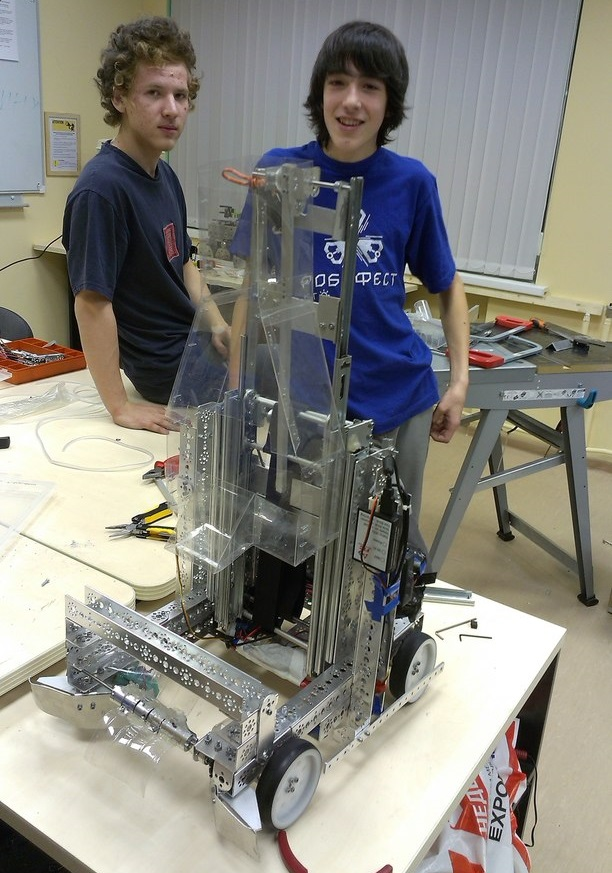
\includegraphics[scale=0.22]{days/09.01.15/images/01}}
        		\caption{Робот с установленным ковшом}
        	\end{minipage}
        \end{figure}
		
        \item Неподвижный желоб, который будет располагаться в верхней части подъемника для того, чтобы мячи ищз опрокинутого ковша скатывались по нему  и попадали в корзину (в дальнейшем он будет называться "желоб"), было решено сделать из листа оцинкованной стали толщиной 1 мм. На следующем занятии было решено сделать чертеж будущей детали, а затем изготовить ее.
        
        \item Поскольку все аккумуляторы оказались разряжены, нам не удалось протестировать программу управления движением робота.
        
	\end{enumerate}
	
	\item Итоги собрания:
	\begin{enumerate}
		
		\item Сломанная направляющая заменена.
		
        \item Ковш установлен.
        
        \item Протестировать программу управления движением робота не удалось.
		
	\end{enumerate}
	
	\item Задачи для последующих собраний:
	\begin{enumerate}
		
		\item Изготовить и установить пластину, соединяющую вал сервопривода с осью и ведомой шестеренкой.
		
		\item Сделать чертеж желоба и изготовить его.
		
        \item Испытать управление движением.
			
	\end{enumerate}
\end{enumerate}
\fillpage
